\documentclass[]{article}

\usepackage{xargs} 
\usepackage[colorinlistoftodos,prependcaption,textsize=tiny]{todonotes}
\newcommandx{\unsure}[2][1=]{\todo[linecolor=red,backgroundcolor=red!25,bordercolor=red,#1]{#2}}
\newcommandx{\change}[2][1=]{\todo[linecolor=blue,backgroundcolor=blue!25,bordercolor=blue,#1]{#2}}
\newcommandx{\info}[2][1=]{\todo[linecolor=OliveGreen,backgroundcolor=OliveGreen!25,bordercolor=OliveGreen,#1]{#2}}
\newcommandx{\improvement}[2][1=]{\todo[linecolor=purple,backgroundcolor=purple!25,bordercolor=purple,#1]{#2}}
\newcommandx{\thiswillnotshow}[2][1=]{\todo[disable,#1]{#2}}

\usepackage{graphicx}
\usepackage{auto-pst-pdf}
\usepackage{graphviz}
\usepackage{microtype}
\usepackage{enumitem}

%not allowed to call it "Seize them, my minions"
\title{Command Language for Single-User, Multi-Robot Swarm Control}
\author{Abraham Shultz}

\begin{document}

\maketitle

\begin{abstract}

\end{abstract}

Methods for command and control that are based on issuing individual orders to individual robots do not scale to large numbers of robots \cite{WangSearchScale}.
By defining a mapping from user interface gestures to individual programs loaded on each robot, we can allow an individual to control arbitrarily large, heterogeneous swarms.
Previous work in HRI shows that multi-touch interfaces allow a scalable and direct mapping between the desires of the user and sequences of commands to the swarm \cite{micire2009multi}. 
While swarm hardware is not yet at a point where very complex computation may be pushed directly to the swarm nodes themselves, that time is not far off. 
Until computational power in the individual swarm units does reach the levels required for complex computation, virtualization of computing resources can provide an adequate test environment for the development of swarm control algorithms at modest requirements in terms of space and power consumption. 
Centralizing the control of a large group of robots (a swarm) makes the system as a whole sensitive to the failure of the central controller. 
To avoid this type of failure, the overall action of the swarm should be guided by decentralized emergent behavior, rather than a centralized orchestration. 
Each robot receives its own program, and the sum of the execution of the programs on each robot results in completion of the task.
The various approaches to development of swarm robot control programs show that a wide variety of approaches can still result in robust controllers for swarm robots. 

\section{Intro/Research Statement}

\subsection{Problem Statement}

One potential method to control a swarm of robots is having a central computer dictate to individual robots how the robots should move.
However, centralized control is only as robust as the central controller. 
Distributed control systems do not have the single point of failure that centralized models have. 
In order to create reliable and useful swarm robotic systems, users must be able to specify a desired end state of the system that the swarm can converge to without reliable orchestration from a central controller. 
Moreover, this convergence must occur in the face of unreliability on the part of the individual swarm members. 

The current state of development of emergent control of swarms is guided by ad-hoc, iterative development models that are somewhat suited to software developers, but not suited to use by non-programming end users \cite{palmer2005behavioral}.
The motivating examples of uses for swarms are task oriented, such as sending swarm robots into disaster zones to search for survivors. 
While first responders are frequently trained in many specialized skills to perform their jobs, adding programming swarm robots to their training would be impractical. 
Even if first responders could be expected to develop software in a disaster zone, the situation frequently develops faster than the build/test cycles of software development can react. 
It is desirable to automate the construction of control software for a swarm so that it can adapt to a situation, without requiring significant development time. 
In order to support interactive control during a developing situation, the construction of the software should occur over a similar time scale to the user interactions.
Another possible example of an application for swarm robotics is cleaning, whether in a user's house, or in a more hazardous contaminated area. 

In either case, it is desirable for the user to be able to release the robots into the region with minimal oversight, and rely on the robots to discover what areas need cleaning, and to allocate robots to clean them. 
Modern household cleaning robots, such as the Roomba, are restricted to floors, and even specific types of flooring, but a heterogeneous cleaning swarm might include robots for cleaning windows and dusting surfaces as well. 
Currently, this kind of whole-house cleaning does not require programming the cleaning tools in advance, and any product which does require such a task is unlikely to succeed in the market. 

In order to remain useful in real-world applications, this work makes certain assumptions about the robots and the swarm. 
Networking between the robots is expected to be unreliable. 
Individual robots have limited transmission power over radio or infrared light links. 
Network links are also frequently attenuated by distance or intervening objects. 
As a result, when robots spread out into an area, some robots may not be directly reachable from others. 
Any software that purports to control a swarm under these conditions cannot rely on perfect connectivity for its operation. 

Robots' perception of their environment is frequently limited. 
Objects can block the sensing field of sensors.
Even without obstructions, most sensors have a limited effective range.
Because the real world is dynamic, robots can make only limited assumptions about what they cannot sense, and can only sense a limited area. 
Algorithms to control robots must primarily make use of locally sensed information, and secondarily make use of information received in communications from other robots. 

Because of the limited range of their sensing and networking, the localization of the robots may also be unreliable. 
GPS provides a global coordinate system in which robots can easily localize, but GPS signal is absent indoors, under dense tree cover, and in many other areas where it would be desirable to use swarm robots. 
The GPS signal is also weak, and so can easily be jammed by ambient RF interference or by malicious actors. 

Robots can also fail. 
The harsh conditions of the WTC rubble pile destroyed many of the robots sent in \cite{Micire02analysisof}.
In order to remain robust in the face of failures, algorithms should not be developed to depend on the perfect functioning of any individual robot. 
Rather, the behavior should emerge from the interaction of multiple, interchangeable robots, and tolerate the loss of individual robots up to some limit. 
In a situation where many or all of the robots attempting to complete a task are destroyed or disabled, it would be unreasonable to expect the task to be completed, but ideally, the bounds on how many robots are required to complete the task should be knowable. 

%A reliable robotic system is one that performs the required task, within some set of constraints, despite failures of some parts of the system. 
Cooperating systems can be broken down into two major classes, those that intentionally cooperate, and those that coopererate in the manner of ants or other swarm insects, without explicit agreements and planning \cite{parker1998alliance}.
The swarm-like approaches generally assume that the robots are homogeneous and all have the same control software. 
For the work described in this proposal, it may be that neither of these assumptions hold. 
The proposed hardware enables the creation of highly heterogeneous swarms, including variation in scale of the robots involved. 
Because the proposed control software generation scheme is intended to potentially result in different software for each robot, even robots with the same hardware may have different control programs. 
%However, the frameworks for analysis of explicitly cooperating multirobot systems may also not be applicable. 
%It is the intent of this project to have minimial explicit interrobot communication, which precludes many methods used to mutually plan tasks. 

%TODO: investigate CEBOT work 
%TODO: Is it possible to have the compiler compile to ALLIANCE specifications of task ability for each robot? Still has problems with sensing that task is done or other robots are doing it.
%TODO: ALLIANCE doesn't have an idea of minimum robots needed because even one robot can do the job, just more slowly. 
\subsection{Hypothesis}

There exists a number of robots beyond which users will transition from treating robots as individuals to interacting with the robots in small groups or as a single large group. 
This transition point will be apparent because of a change in the gesture set that the user uses to interact with the swarm. 
It is hypothesized that above the transition point, users will be more likely to neglect some subset of the available robots. 
The user will instead use commands that control the bulk of the robots as a cloud or flock, but may leave some robots unused. 
For example, the user may switch from selecting robots as individuals to shaping and pushing the swarm the way a child might play with a bug, putting their hand down so the bug goes around or avoids it, touching the back of the bug gently to make it scurry forwards, and so forth, or by shaping the group as if sculpting, with pushing and pinching to ``carry'' groups around. 
The user may also change how they indicate which robots are to be interacted with. 
Rather than selecting each robot by clicking on it, the may ``paint'' over the area containing the robots they want to use, or draw a circle around them. 
The size of the swarm where changes in the user gestures occur will indicate the transition point between the user intent to interact with individual robots as opposed to interacting with the swarm as a whole. 
%Harriet \emph{et al}. also put the estimated transition point between multi-agent control and swarm around 50 individuals \cite{harriott2014biologically}.  
%Above that threshold, human interaction may be able to remain focused on macro level behavior, influencing the overall behavior of the swarm rather than control of individuals.
%TODO is this relevant, if so, how?

Once the ratio of the size of individual swarm members to the size of the area the swarm is in becomes sufficiently large, displaying the swarm members at the same scale as the map will result in the representation of the swarm members being too small to interact with. 
This problem will arise at smaller scales if the swarm robots are themselves quite tiny, and some of the available swarm robots are indeed small \cite{pelrine2012diamagnetically}.
Scaling the representation of the robots up, relative to the map, will make the robot representations overlap unrealistically and obscure the map. 
Instead, we propose that for certain scales of swarms, it makes sense to represent the swarm as the area covered, rather than the locations of the individual robots.
This approach has been used successfully for navigation in three dimensions, by developing a controller that causes the individual UAVs to remain within a bounding prism, and allowing the user to control the shape and location of that prism \cite{ayanian2014controlling}.
Altering how the user interface displays the location of the robots in the swarm will affect the transition point. 
More specifically, a display which obscures individual robots and displays a cloud or swarm boundary will cause the user to treat the swarm as a whole rather than individuals, which will be apparent because the user will use different gestures. 

Further, it is hypothesized that it is feasible to convert user commands into programs for each robot which will converge to the desired behavior using only local sensing and local communications, and without resorting to global, absolute localization. 
However, this hypothesis must be modified with a few caveats. 
First, under the assumption that robots can fail, it is possible that the entire behavior can fail. 
For example, if enough of the robots are incapacitated, it may be that not enough are left to complete the task. 
It's also possible that at compile time, the task is still possible, but a later change of the environment renders it impossible. 
Assessing whether or not a user-specified action will be completed is not possible for all of the usual reasons that prevent prediction of the future, but in some limited cases, it may be possible to determine whether a specified action is impossible. The goal of this work is to provide a best-effort attempt to satisfy the user command, rather than prove anything about the possibility of doing so. 

%(Hadas http://link.springer.com/chapter/10.1007/978-3-642-22110-1_54#page-1 makes a distinction between unsatisfyable and unrealizable specifications. Unsatisfyable specs are those that the robot cannot do in any environment. Unrealizable specifications are those cases where there exist environments that can thwart the robot. In Hadas' work, there's also the idea that environments are finite in number. )
%\unsure{``Best effort", based on the information available, it's worth an attempt vs. not worth an attempt.}
%\unsure{So since we can't tell if a program will succeed, and determining if it is impossible might not be tractable, how do we know if we've written a compiler that does this?}

\section{Related Work}

\subsection{Overview of Previous Swarm Hardware}

Swarm robots are generally small. 
The reason to keep swarm robots small is related to both the cost of making them and the cost of using them. 
Larger robots consume more materials per unit, and so cost more money.
As a result, for a given number of swarm units, larger robots will result in a higher cost swarm. 
Also, each robot requires some amount of space to move around in. 
To keep the ratio of free space to robots constant, the area of space used by the robots grows as the robots do. 
If the ratio isn't kept constant, the robots will crowd each other, and so large robots will require either a very large space, or become overly crowded.
Finally, larger robots are more cumbersome to deal with. 
They require larger storage areas, possibly teamwork to lift or repair, and so forth. 
All of these efforts are also multiplied by the number of robots in the swarm. 

The robots used in most swarm work are of a sufficiently small size that many of them can fit in a room. In addition to budgetary constraints, interaction with an environment built for humans places an upper bound the scale of the individual swarm members. 
For example, typical indoor doorways are around thirty inches wide, so a robot would have to be less than thirty inches wide to fit through them. 
The lower bound on swarm robots is generally dictated by fabrication technology, with smaller robots becoming increasingly difficult to assemble. 
As a result of these bounds, swarm robots are mostly between 1cm$^3$ and 0.3m$^3$. 
This scale range divides fairly evenly into robots that can operate in large swarms on a table, and those that can operate in swarms within a room, albeit possibly a large room. 
The challenge of construction of swarm robot hardware, then, is to put all of the same parts as non-swarm mobile robots: a mobility platform, a power supply, a processor, some sensors, and a communication system, into a small package.
Many impressive designs for small swarm robot platforms have been proposed and constructed as part of research in swarm robotics. 
However, most of these platforms are no longer easily commercially available, or never were. 

\subsubsection{Tabletop Swarms}

At the low end, in terms of size, the I-SWARM Project was intended to create a 2x2x1mm robot that moved by stick-slip locomotion actuated by piezo levers \cite{seyfried2005swarm}. 
Over the course of the project from 2004-2008, the hardware was developed and used in research, but was not converted to a commercial product.
Other techniques have been developed to use magnetic fields to apply force to small magnetic objects, resulting in controlled motion of the objects \cite{floyd2008untethered, pelrine2012diamagnetically}.
These systems are not amenable to decentralized control, because the moving components are not themselves robots. 
The moving parts are more accurately viewed as manipulators, with the instrumented environment, any sensors for feedback from that environment, and the manipulators themselves comprising a single robot. 

Alice, by Caprari \emph{et al}. \cite{caprari1998autonomous} combined a PIC16F84 processor, motors, RF and IR networking, and enough battery power for 10 hours of autonomy into a robot measuring under 2.5cm$^3$. 
The processor used in Alice is relatively underpowered compared to modern processors at the same price point and power consumption. 
Alice robots are no longer available for purchase. 
The AmIR robot was similar to Alice in size and capability, but with a more modern processor \cite{arvin2009development}.
There is no evidence that AmIR was ever widely available.

The Jasmine swarm robots were possibly the closest thing to a commercially-available successor to Alice  \cite{kernbach2011swarmrobot}.
Jasmine measured 26x26x20mm, and included an ATMega processor, IR close range communication and obstacle detection, two motor skid steering, and li-po batteries.
Unfortunately, Jasmine units cost about 100 Euro (\$111 USD) each when they were available, and they are no longer available for purchase. 
The plans and information required to reproduce Jasmine units are available for free at Swarmrobot.org.
Assembling a Jasmine robot is not beyond the reach of competent electronics hobbyists, but it does require some unusual build processes, such as grinding down the cases of certain electronic parts and filling holes in the PCB with solder to prevent light leaks. 
The chassis of Jasmine is also a custom mechanical assembly, rather than a commercially available product. 

InsBot was a small robot, measuring 41mm x 30mm x 19mm, that was designed to interact with cockroaches \cite{colot2004insbot}.
It used two processors, one to run higher level behaviors and one to interface with a suite of sensors that included 12 IR sensors and a linear camera. 
InsBots were never commercially available, and each required approximately 6 hours of work to assemble by hand. 
However, the construction process appears to have been relatively straightforward. 

Even when they are commercially available, most existing swarm robots are too expensive to build a large swarm.
The Epuck from EFPL is approximately 800 Swiss francs (\$810 USD) per unit, so the cost of maintaining a large swarm can become daunting quickly. 
The high price of the Epuck is a result of its extensive suite of sensors, including a camera and 360$^{\circ}$ IR range sensor and communication system. 
Epucks also require a fairly smooth operating surface.
The Epuck uses differential drive, and allows the front or back edge of the robot to serve as a skid. 
Due to the relatively sharp corner of the lower edges of the robot, the Epuck can become stuck on 2-3mm high obstacles. 

The r-one research robot is cheaper than the Epuck, at approximately \$220 USD per unit \cite{mclurkin2013low}. 
The developers of the r-one position it as a more-featureful and less expensive alternative to the Epuck (\$810, cannot sense neighbors without additional hardware), Parallax's Scribbler (\$198, minimal sensors), the iRobot Create (\$220, requires additional hardware to be programmable), the K-team Khepera III (\$2000), and the Pololu 3pi (\$99, minimal sensors). The main advantage in sensing that the r-one has over these other platforms is neighbor sensors and ground truth position sensing, both of which are implemented on the r-one using infrared.
The design of the r-one is open source, but it does not appear to be commercially available as of this writing.   

The Harvard Kilobots are a more recent entry to inexpensive swarms, and have been produced in large quantities \cite{rubenstein2014kilobot}. 
Kilobots contain about \$15 worth of parts, but a 10-pack sells for 1100 Swiss francs, or about \$112 (US) per robot. 
The Kilobots are intended for research in a highly homogeneous environment, with most or all of the robots executing the same program. 
As a result, they are designed to be programmed in parallel using an IR interface. 
For small groups, individual Kilobots can be programmed differently, but any attempt to give each of a very large collection of robots an unique program will take a long time. 
The Kilobots also move by stick-slip motion, and so must operate on a smooth surface, such as a whiteboard. 

One way to reduce the cost of swarm robots is to use commercial, off-the-shelf (COTS) hardware in the construction of the robot. 
Reusing existing hardware leverages the economies of scale that reduce the price of commercial hardware, as well as eliminating the need to design or build the COTS parts. 
Use of COTS parts in research robotics has led to at least two platforms referred to as COTSBots \cite{bergbreiter2003cotsbots, soule2011cotsbots}.
The first COTSBots used mote hardware for the communications link and sensing, plus a motor control add-on board \cite{bergbreiter2003cotsbots}. 
The mobility platform is a modified toy, in particular, a specific brand of high-quality micro RC car.
At the time of this writing, the car used in COTSBots is moderately expensive for a toy car, although quite cheap for a research robot, costing a little over \$100USD per unit. 
COTSBots use TinyOS, a modular and event-driven framework for developing node software \cite{levis2005tinyos}. 
TinyOS is written in a dialect of C called nesC. The motor and mote boards communicate using a messaging layer. 
The motor driver board is not commercially available, but can be custom-built by board fabrication companies, without the researcher having to assemble it by hand. 
The second COTSBots is larger, and will be discussed in the next section. 

\subsubsection{Room-sized Swarms}

One potential problem with extremely small swarms is that while the robots may scale down, the scale of obstacles they have to traverse may not scale with them. 
As previously mentioned, the Kilobots require a smooth surface, and the Epuck can be stopped by obstacles no more than a few millimetres tall. 
This sort of vulnerability prevents the smaller, tabletop swarm robots from operating well in human-scaled environments. 
In order to overcome this problem, larger swarm robots can be constructed.
 
The MarXbot swarm platform is capable of operating in unstructured human environments. 
MarXBots can also use their grippers to link themselves together and perform operations that an individual robot could not perform, such as bridging a gap larger than a single robot \cite{bonani2010marxbot}. 
The size and complexity of the MarXbots, as well as their powerful computer, renders the individual robots quite expensive. 

Swarmanoid extends the interlinking mechanism of MarXbot to a heterogeneous swarm with three different types of robots \cite{dorigo2013swarmanoid}.
The ``foot'' robots are MarXbots, and provide ground motion for ``hand'' robots. 
``Hand'' robots have grippers to manipulate objects, and can also climb.
The ``hand'' robots have an attachment point like the MarXbots, and so can be carried by ``foot'' robots. 
Flying ``eye'' robots provide overviews of the work area and networking.  

In order to reduce costs, another platform called COTSBots was developed \cite{soule2011cotsbots}.  
Instead of sensor motes on micro-scale RC cars, the newer COTSBots platform is composed of a laptop for processing and a modified RC car, tank, or similar toy as a mobility platform.
In order to interface between the laptop and motor drivers, a second micro-controller board, such as an Arduino or Phidget interface, may be used. 
Due to the diversity of possible combinations of hardware that can be assembled into this configuration, it is still a very viable platform. 
However, the minimum size of this style of COTSBot is the size of a laptop, which is in turn dictated largely by the minimum size of a useful keyboard. 
The large size of these COTSBots demands a very large space if the density of robots in a large swarm is to be kept low. 
Additionally, each laptop has a screen, keyboard, and so forth that are not useful while the robot is operating. 
All of these parts add to the overall cost of the swarm. 

Beyond the scale of rooms, swarm research has been done with Amigobots and Roombas, as well as larger custom platforms for outdoor multi-robot work \cite{guo2007bio, tammet2008rfid, olson2013cacm}.
In theory, swarm research could be performed using robots of any size, but financial limitations would place it out of the reach of most academic organizations. 

\subsection{UI Designs}

The user interface to a swarm has two functions. 
The first is to allow the user to provide input to the swarm, so that the user can direct the swarm to perform tasks. 
For the purposes of this research, the user interface is a multitouch surface that displays representations of the area the swarm is in and of the individual swarm robots \cite{micire2009multi}. 
The second function of a swarm user interface is to display information about the swarm, or to display information gathered by the swarm to the user. 
By providing an overview of the activities of the swarm, the user interface can give the user feedback on the progress of the task as it proceeds, as well as allowing the user to detect problems. 

Multitouch interfaces have been determined to improve on WIMP or voice interfaces for multi-robot control in a sequence of command and control tasks, including commanding the swarm to a location, performing reconnaissance, and having the swarm cross a dangerous area \cite{hayes2010multi}.
The interface displayed the locations of the robots on a directly manipulatable map, and used movable or semi-transparent user interface widgets, in order to minimize occlusion of the map. 
Areas were selected with with drawing gestures, and paths with fluid strokes, rather than e.g. selection of vertices bounding an area.
The use of multi-touch interaction is desirable because one-at-a-time selection doesn't scale beyond a very limited number of robots.
In order to interact with large groups of robots, the user must be able to perform operations on areas and groupings, rather than on the single point available with a traditional pointer-based interface. 

One approach to getting feedback from a swarm was the development of the Swarmish sound and light system \cite{mclurkin2006speaking}. 
Swarmish provides an ambient means of determining the overall state of the swarm, as well as some information about individual robots. 
The swarm that used Swarmish had autonomous charging, and so the individual robots had long runtimes, and minimal one-on-one interaction with humans. 
As a result, most of the interactions were remote.
The ``ambient'' aspect of the interaction is that the information is continuously available, and the human user ``tunes in'' to it when needed. 
Swarmish uses a set of colored lights and sounds, produced by each robot, to provide feedback. 
The lights were in three colors, and had a total of 108 different combinations of colors and blink sequences, as a visual indicator of the state of each robot. 
In addition to the lights, each robot could produce MIDI notes over its audio system. 
Each note can vary in instrument, pitch, duration, and volume, in addition to having tempos and rhythms as the code executes. 
The designers of Swarmish indicate that the sum of the audio output of the swarm could provide a overall idea of the status of the swarm, but that as a musical instrument, it is difficult to play well. 
Further, the use of lights as signaling mechanisms assumes that you can look at the robots. 

If we accept the assumption that the robots are visible to the user, the robots can carry some form of display that provides local information to the user. 
This information can then be displayed as an overlay in the real world, with the display of the information conterminous with its presence \cite{Daily:2003:WEI:820752.821587}. 
Local display of local information works if the user is part of a hybrid human/robot team, and so is in the same location as the users. 
However, there are many situations where the robot is not in the same location as the user. 
A common example is urban search and rescue, where buildings may be known to be unsafe, or of unknown stability, but it is desirable to search them for trapped people. 
In such a situation, the human user would rather be located elsewhere, and receive information from the robots. 

For situations where the user is not located in the same area as the robots, one possible approach is a ``call center'', where robots can request human attention when required \cite{chen2011supervisory}. 
The human in the call center, however, is faced with having to answer potentially multiple calls with no awareness of the robot's situation. 
The theoretical basis for call center UI is Supervisory Control. 
Supervisory control has the human act as the planner and monitor of the systems being supervised, but allowing the systems to operate on their own.
Automation is frequently broken down into ten levels of automation, with level 10 being a fully automatic system with no humans involved, and level 1 having no automation, such as a bicycle \cite{parasuraman2000model}. 

It would be expected that reducing the number of times the human is required to interact with the robot will permit the user to operate more robots.
At level 1, the user has to interact constantly, and so could not be expected to operate more than one robot. 
By increasing the level of autonomy of the robot, the time required for the user to operate the robot decreases.
Instead of continuous interaction, the user can specify actions for the robot to undertake, and then ignore the robot while it performs the actions.
It is expected that the robot's effectiveness will decline over time since the last user interaction. 
This time that the robot operates without interaction before its effectiveness declines to a fixed minimum is called ``neglect time"\cite{olsen2003metrics}.
With increasing autonomy, neglect time increases.
The fifth level of the autonomy scale is a sort of operation by consent model, where the computer chooses a route and executes it if the human permits it. 
The ninth level is the inverse of the fifth.
Rather than asking the user for consent to act, the robot acts and informs the human only in exceptional cases. 
At the higher levels of the autonomy scale, the robot's neglect time far outweighs the time the user is expected to operate it, and so the user could reasonably be expected to operate other robots during the neglect time. 

Increasing neglect time may allow the user to operate more swarm robots, but it comes at a cost. 
The longer a user goes without learning about the state of one of the robots, the less idea they will have of the situation when they are called upon to operate that robot. 
The problem of automation decreasing the situational awareness (SA) of the user has been described in cockpit automation for aircraft \cite{wiener1980flight}, and generalized well to other systems that combine automation with human control \cite{kaber1997out}. 
If the user takes a long time to relearn the situation, the efficiency of the system will drop. 
Worse, the user may make errors because of an incorrect understanding of the system when they begin operations after a long neglect time \cite{cummings2008predicting}. 
One possible approach to maintain a constant and manageable workload on the user is adapting the level of automation to the workload. 
When the load is low, the user is more directly engaged, but when load is high, there is more automated assistance. 
By varying the level of automation, the workload for the user is kept constant. 
A constant workload is desirable because the user remains engaged with the work, and so has an ongoing understanding of the situation as it develops. 
The user is not suddenly called into a situation after remaining disengaged for some time. 
However, the workload must also be manageable. 
If the user is overloaded, their attention will become subject to triage, and they will begin to miss elements of the task. 
Adaptation does not have to be based on measured load, but could instead be based on perceived load or physiological markers in the user. 
%\cite{goodrich2010maximizing}

However, in situations with even moderate numbers of robots, even relatively high levels of automation may overwhelm the user \cite{lewis200617}. 
Level five, operation by consent, is a fairly high level of autonomy, but with a large number of robots checking in, even this level may generate too many events for the human to deal with. 
Increasing the autonomy to level nine, so that the robots are only checking in with the operator when an exceptional situation occurs, may still overwhelm the operator if enough robots are active.
Increasing the use of automation may also create new difficulties by leaving operator out of practice, or encouraging mis-placed trust in the automation's ability \cite{lee2004trust}. 

In fact, any kind of multitasking may prove insufficient for large swarms. 
For teleoperation, the best case is uncrewed aerial vehicles (UAVs), which require relatively little oversight. 
Uncrewed ground vehicles (UGVs) require more oversight than UAVs, due to the higher complexity of the ground environment. 
Estimates place the limits on the number of robots under control at 12 or 13 for UAVs and 3-9 for UGVs \cite{WangSearchScale}.  
There is some latitude, at least in UGVs, to increase multitasking by increasing automation, as shown by the relatively wide range in the interaction limits, but even 9 robots per operator is nowhere near the scale of kilo-robot swarms  \cite{Olsen:2004:FMH:985692.985722}.
Failure generally takes the form of task effectiveness no longer increasing as more robots are added.
Instead, the amount of time the user spends interacting with the robots begins to outweigh the neglect time, and so the robots spend increasing amounts of time waiting for interactions \cite{cummings2008predicting}. 

Ecological interface design (EID) presents a possible guide to the architecture of user interfaces for swarm robotics, and has been used in interfaces with mixed human-robot teams \cite{vicente1992ecological, gancet2010user}. 
In EID, a user's abilities that enable them to interact with a system is separated into a taxonomy of skills, rules, and knowledge. 
The user has skills, which are rote, simple activities that form the basis of the normal operation of the system. 
The user also knows a set of rules about the system. 
Rules allow the user to handle exceptions or unusual cases that have come up before. 
Rules do not require the user to understand the system, just to know that when certain situations are recognized, certain actions must be performed in response. 
Beyond rules and skills, the user also has knowledge of the system. 
Knowledge allows the user to handle novel exceptions. 
Knowledge gives the user an understanding of how the system works, and can apply that understanding to react to situations that the user has not experienced or been told about before. 
Events are also broken into three levels: routine, which uses skills; foreseen exceptions, which use rules; and unforeseen exceptions, which use knowledge. 
All levels should be supported by the interface, but the user should not be forced to operate at a higher level than is required. 
The abstraction of the process maps onto the hierarchy of ecological design, with the highest level being the function of the process and the lowest level being how the function is accomplished. 
At each level, there are constraints on the process that are used to define the normal operation of the process.
Detection of exceptions requires the display of all constraints, because exception is the breaking of constraints, and undisplayed constraints cannot be assessed to determine if they have been broken.

The user should be able to extract meaning from the information display quickly, as in the case of Swarmish and the robot-as-pixel UI designs.
By using the lights in Swarmish, the user can assess the state of individual robots, but by listening to the overall sound of the swarm, the user can also assess the behavior of the system as a whole.
The state and status lights of an individual robot is the low level in EID, watching how an individual action of the overall process is progressing. 
The ``tune'' of the entire swarm, produced by the sum of their MIDI notes, provides the high level overview, where a user can tell if the system is progressing well or developing problems. 
As the system changes, the changes and predictions should be highlighted so that the user understands consequences of their actions. 
In Swarmish, sudden changes in the tone or tempo of the swarm tune indicate transitions in its behavior, without the user having to observe the actions of the robots closely. 

EID is well-positioned to deal with emergent behavior, because the emergent behavior of the entire system is present at the functional level, but is composed of actions at the physical level.  
The control of swarm robots can be viewed as a hierarchy of increasing abstraction. 
At the least abstract, base level are the individual interactions of the swarm robots with each other and their environment, as dictated by their explicit programs. 
Above that level is the implicit, emergent behavior of the swarm as a whole. 
Finally, the most abstract level is the user intent, as expressed in the interface through their gestures. 
This hierarchy corresponds well to the abstraction of process in EID, with discrete physical actions at the lowest level and the overall results of the process at the highest level. 
Consequently, the user is permitted to issue commands in the most abstract domain, and the system can propagate them ``downwards'' into the concrete actions of the robots in the world, while also propagating information from individual robots ``upwards'' into the global view. 

Automation in EID allows the user to operate primarily with rules and knowledge, dealing with exceptions \cite{vicente2002ecological}.
The interface should allow direct manipulation of perceptual forms that map directly onto work-domain constraints and represent all of the information identified by the abstraction hierarchy. 
In a swarm context, this means displaying functional information in such a way that the user can move across the hierarchy from individual swarm bots to high-level swarm-wide tasks, and interact at all levels to control the swarm. 
More practically, this means that the information displayed must be integrated in such a way that the mapping from one unit of information to another is made apparent in the interface, rather than offloaded to the user to compute in their head \cite{yanco2004beyond}. 
For example, if a robot can send video and range information, the video and range information can be projected into a 3D space around the robot, rather than being displayed in separate UI windows.
Such a projection allows the user to easily relate visual and range information, and relate that information to the ongoing robot control task, which in turn increases task performance \cite{ricks2004ecological}.
Previous work in multi-touch interfaces directly satisfies these requirements of EID by providing both an omniscient camera view for direct manipulation of the high-level, functional actions of the entire swarm, and the ability to move down the hierarchy to control individual swarm members \cite{Micire:2009:ANG:1731903.1731912}.
The ability to display information about individual robots along side or on top of the interface representation of the robot is an important method of providing feedback to the user \cite{Kato:2009:MIC:1520340.1520500}. 

% TODO: Maybe use some of this stuff, but I don't have a good idea where
%Emergent behaviors arise from the interactions of actors with each other and the world around them. 
%In the face of uncertainty in the world, the behaviors will also become uncertain. \change{cite trust work}
%Programs synthesized to guide the swarm should be designed to be robust against failure or degradation of swarm members. 
%The heterogeneity of the swarm may also be leveraged to increase its robustness against failures of individual nodes or alterations of the environment. 
%However, because heterogeneity increases the dimensionality of the solution space for program synthesis, it may adversely affect the performance of the program synthesis and the swarm's runtime convergence to the desired state.
%
%A concept of the swarm as a whole as a programmable entity runs into trouble with reliability. 
%In conventional compilation, assuming the compiler is correct and the computer is correct, the compiled binary does what the source code says. 
%Robots interact with the real world, which is much less likely to be ``correct'' in the same sense a compiler can be asserted to be. 
%Programs for swarms are only going to be functional within some probabilistic grounds and assumed conditions. 
%This requirement indicates that the situation has to be at least somewhat known ahead of time, so that the robots will all receive programs that allow them to perform the task.
%In the ideal case, the emergent action of all of the robots interacting with the environment causes them to perform the task. 
%
%Swarms have more uncertainty, because the reliability of individual robots is low; and higher attentional demands because there are many robots. 
%It may be that above some threshold, the attentional demand will drop again, as the group is no longer treated as a large number of individuals, but as a single group. 
%%A lot of Dr. Adams' work in HSI was under ONR Award N00014-12-1-0987
%
%If the user is unconcerned with the functioning of individual swarm members, so long as the swarm as a whole remains functional, the UI may simply drop malfunctioning individuals from view. 
%This handling of error conditions on individual swarm units fits with the assumption that the swarm as a whole achieves robustness through redundant expendable units, while also allowing the human user to have a rough idea of how the situation is developing by watching the cloud shrink. 
%Do long as progress appears to be being made on the mission, the user might let underperforming units slide. 
%The supervisory system might not even announce when units are lost, until it starts to affect performance.  

\subsection{Swarm Software Development Methods}

Because the conversion of the specification of desired behavior for the swarm into individual programs for the swarm member robots is still an open question, it is necessary to understand the current methods used in the development of programs for swarm robots. 
Much of swarm robotic development follows the usual model of software development. 
Starting from a desired functionality, the developer writes a program that they think will provide that functionality.
The program is then tested, in simulation or on real robots, and its behavior is observed. 
The programmer then modifies their program to account for any observed difference between the desired function and the system's behavior. 
This loop of coding, testing, and coding again is repeated until the system behaves as expected, or the programmer graduates. 

Because the normal software development model is time-consuming, and outside of the abilities of many people who might want to use swarm robots, it is desirable to automate the development of software controllers for robots. 
One approach to the conversion of the command language to programs for the robots is to define a transformation from the command language to executable code that can be codified into a compiler. 
As a consequence, input in the command language defines a program which is compiled and loaded onto the robots. 
Another possibility is the composition of preexisting behaviors that each satisfy part of the user's desired behavior. 
Pheromone robotics provides one possible method of controlling this composition dynamically. 
Still another approach is to allow the user to specify a desired behavior and evolving controllers to match it. 

\subsubsection{Amorphous Computing}

Amorphous computing (AC), also called spatial computing, is computation using locally-linked and interacting, asynchronous, unreliable computing elements dispersed on a surface or throughout a volume \cite{abelson2000amorphous}. 
The motivation for AC is that while it may be possibly to produce arbitrary quantities of ``smart dust'', it is not possible to ensure that it all works well and is precisely located, especially in real-world applications.
The goal of AC is to get useful work out of such materials, despite uncertainty as to their reliability and location. 
Smart dusts are also the limit-case, in terms of scale, for swarm robotics, and if AC promises to get useful work out of smart dust, then it also has some applicability to larger swarm robots.

There are several languages intended to program amorphous computers. 
``Proto" is a language for a continuous plane spatial computer \cite{correll2009ad}.
Because the devices are distributed over a plane, the difficulty in communicating between any two devices is a function of the distance between them, much as with RF or other radiative communications.
In Proto, the behavior of regions of space is described by the programmer, and the description is transformed into local actions for the network of devices. 
Because devices have a size in the real world, and space between them, the devices cannot not have a one-to-one mapping with the space, but instead perform an approximation of the desired behavior. 
Swarm robots are mobile, so some swarm algorithms can be implemented as a description of constraints on the robot's state, such as ``the robot must have communications links to no more than 2 and no less than 1 other robots", and a command to move randomly unless the constraint is satisfied. 
Within a bounded environment, such an algorithm can be shown to converge to satisfy its constraints \cite{correll2009ad}. 

Proto also has considerable appeal as a programming language for swarm control development because of the layering in its structure. 
Proto is designed to map from behavior of regions at the global level to programs for discrete points at the level of individual devices \cite{beal2006infrastructure}. 
If user interface interactions can be interpreted as indications of desired behaviors displayed over spatial regions, then conversion of those behaviors into programs in Proto may be amenable to automation. 
Proto's layered structure also has a clear relationship to the hierarchical structure of EID, with the programming language serving as a user interface at the highest abstraction level of the interface design, but providing a smooth transition to the lower abstraction levels.  

Origami Shape Language (OSL) uses the abstraction of a foldable sheet to form shapes, inspired by both origami and the folding of epithelial cells during the development of biological organisms \cite{nagpal2004engineering, nagpal2001programmable}.
Regions and edges on the sheet can be defined by propagation of morphogens, and folds along the edges result in the development of the final form.
Because of the use of morphogens and local communication between the agents on the sheet, there is no need for a global controller to dictate the development of the final form. 
Further, because the high-level description of the desired form does not involve abstractions of the underlying modules, OSL could operate on interlocking modular robots, actuated flexible materials, swarms, or other kinds of computational media. 
In fact, the flexible sheet could be assumed to be virtual, and the resulting motions of the sheet could be translated into motor commands to configure swarm robots into specific arrangements in space. 

Growing Point Language (GPL) allows the specification of topological patterns in an amorphous computer, and so can also be used to specify the distribution of swarm robots, or behaviors of the swarm robots, in a space \cite{nagpal2004engineering}. 
GPL is inspired by the morphogenic controls present in biological organisms, which use gradients of chemicals called morphogens to dictate the development of cells \cite{turing1952chemical}.
The name GPL arises from one of the language's main abstractions, the growing point. 
The growing point is the location of activity within the amorphous medium, at which local agents are changing their state. 
Growing points move through the medium, affecting the state of the computational points they pass, and emitting pheromones into the medium which control the motion of growing points.

Importantly, GPL does not make any prior assumptions on the location of the particles in the system, or robots in the swarm, aside from that they are sufficiently dense in the medium. 
For swarm robotics, this is an important quality, as precise localization may not be available. 
Initially, all agents have the same state and program, with a few exceptions that serve as seeds for the growth to begin. 
If the pattern is not required to be fixed at a particular location, even the seeds could be undetermined initially, and elect themselves via a method such as lateral inhibition. 
During the execution of the GPL program, each agent chooses its state based on the presence of pheromones, which are morphogens with limited range. 
Range limitation on morphogens propagating between robots is set using a TTL (Time To Live) counter that propagates with the morphogen, and is decremented with each hop in the communication network. 
When the TTL hits zero, the morphogen message is no longer propagated. 
By controlling the production or propagation of morphogens within the amorphous medium, complex patterns can be developed. 

\subsubsection{Pheromone Approaches}

The abstractions of GPL bear a very strong relation to pheromone robotics. 
Pheromone robotics refers to a metaphor for developing control software for swarm robots. 
Some social animals, especially insects, use chemical signals called pheromones to communicate with each other. 
For example, wasps inside their nest react to the scent of wasp venom by travelling to the outer surface of the nest and attacking nearby moving targets  \cite{jeanne1981alarm}.
Ants leave trails of pheromones for other ants to follow to food sources. 
Each individual ant's contribution to the trail can be modulated by the quality of the food source, which allows the reaction of the other ants to the trail to cause an emergent distribution of the foraging work force that favors higher-quality food sources \cite{sumpter2003nonlinearity}.
Because pheromones are chemicals with spatial locations, it would be possible to combine the use of pheromones with reaction diffusion equations to structure activity within a space or to converge to patterns of activity over time  \cite{turing1952chemical}. 
Assuming even diffusion of the robots in space, the global map of the pheromone concentrations is represented over the network by the locally-computed concentrations computed by each robot.

In pheromone robotics, the pheromones are usually simulated or ``virtual'' pheromones, rather than real chemicals which are detected by chemical sensors (for an exception, see \cite{hayes2001swarm}). 
Each pheromone can have properties such as diffusion and evaporation rates that result in the pheromone spreading in space or gradually disappearing. 
In addition to its properties, the pheromones may have other characteristics which robots can sense. 
For example, a robot may emit a pheromone which diffuses into the environment and evaporates quickly, so distance from the robot can be determined by the strength of the pheromone, and approaching or avoiding the robot may be accomplished by moving up or down the gradient of pheromone strength. 
If the swarm is engaged in a search, each searching robot may emit a ``search marker'' pheromone that lingers in the area after the robot leaves. 
Other robots, on entering the area, would detect the pheromone and know that searching this area again would be fruitless. 
If the object of the search can move, the marker pheromone could diminish as a function of time, so areas that have not been searched for a long time become unmarked and may be searched again. 
Once the target is found, the robot may stop and emit a ``discovery pheromone'', which diffuses into the environment, attracts other robots, and causes them to also emit a discovery pheromone. 
As a result, once any robot discovers the target, all of the robots quickly converge on its location. 

The addition of directional communication for the messages that convey virtual pheromone information allows easy determination of the direction of pheremone gradients \cite{payton2001pheromone}.
Rather than directly diffusing in the space as a chemical would, hop counts in the network of robots simulate diffusion. 
Because routes may be of different length, the message with the lowest hop count is assumed to be the truest indication of minimal distance within the network. 
Rather than modelling the world based on the incoming messages, the content of the pheromone messages and the network behavior as a whole serves as a model of the world, mapped 1:1 onto the real environment. 
While it is possible to build a set of behavioral primitives out of pheromone signalling and associated behaviors, controlling the swarm to perform a task with these primitives is still done by hand \cite{payton2003compound}.

In all of these examples, the sensing of the pheromones is assumed to be local to the robot, at least metaphorically. 
To actually maintain pheromones in the environment without robots being present to transmit them requires, again, a global representation of the task space which the robots can refer to when needed. 
Use of pheromones to guide swarm robots for simulated search and patrol tasks has been demonstrated, with the assumption that there is a central controller maintaining the concentration of pheromones on the map, and informing the swarm members \cite{coppin2012controlling}. 
In a real implementation, some robots could remain stationary and only act as transponders, computing and transmitting the local pheromone information for a given area. 
However, even if the robots are limited to only the pheromones they can directly perceive and emit at the present instant, some emergent behaviors are still possible. 

It has been demonstrated that a swarm can perform construction tasks using only local sensing and no communication \cite{wawerla2002collective, bowyer2000automated}.
However, the addition of communication between systems and memory of the state of the world will improve the efficiency of the system.
The system under discussion was developed to have the task implied by the behaviors available for the agents, rather than generating the program from a higher-level specification, such as the form of the structure to be built.

Pheromone approaches can guide the construction of objects, even if the individual swarm members have no memory and only local perception \cite{mason2003programming}. 
The agents engaged in the construction move at random, and take actions governed by their individual perception of environment at present time. 
The agents can release and react to pheromones in the environment, and so there is an implicit communication via stigmurgy, but no explicit agent-to-agent communication. 
The set of rules that govern the mapping of sensor precepts to actions must be such that no point in the construction of the building can be mistaken for another, as that could result in loops or skipping parts of the building sequence. 
The TERMES project created a compiler that translates desired final structures into rules to guide the construction of those structures by cooperating agents \cite{werfel2014designing}.

Both global vector fields and the global and local blending of vector fields in co-fields can be viewed as subsets of pheromone robotics that use a global spatial representation. 
One approach to a control UI for a remotely-located swarm is a multi-touch interface for specifying a vector field \cite{Kato:2009:MIC:1520340.1520500}.
Because the user interface design focuses on the vector field rather than individual robots, the same control interface can scale to an arbitrarily large collection of robots. 
Vector field paths can have loops, which do not exist in waypoint-based paths. 
Waypoint paths have explicit ends, unless an additional command is added to join beginning and ending points. 

Vector field paths have substantial limitations. 
Because the vectors are bound to a 2-D plane, the paths they create cannot cross each other. 
Instead, they flow together. 
A 2-D vector field is also not a useful metaphor for controlling UAVs.
The vector field could be possibly extended into three dimensions, to control UAVs as well as ground vehicles, but there would have to be some form of discontinuity in the field to prevent assignment of UAVs to ground vehicle paths and vice versa. 
The vector field can be viewed as an abstraction of pheromone control, or even implemented in terms of the presence or absence of virtual pheromones, but it has some limitations that pure pheromone control does not have.
For instance, pheromones permit the presence of multiple pheromones at one point, with multiple meanings, but the vector field has one value for each point. 
The vector field is also not very intuitive to users. 
Kato \emph{et al}. indicates that in order to use the vector field well, the users had to anticipate and project the future motions of the robots. 
Interface changes, such as showing particles on the vector field, could improve usability, but these approaches would have the same scaling problems that the robot representation does. 
When the view is zoomed out very far, individual whirls and eddies in the field may not be visible to the user. 

This vector field interface does not directly map to programs on the robots. 
Instead, the central computer maintains the vector field representation and commands the individual robots.
Vector fields also do not allow the assignment of tasks to robots, but allows the user to directly control the motion of the robots. 
In order to convert from a task-based user interface to a vector field representation, the task would have to be converted into a series of changes to the field.
Since the robots may not have accurate localization within the task space, it may not be possible to guide the robots by relating their position to a global vector field. 

The use of co-fields may provide a way to move the vector field representation from the central computer to the swarm, or allow the swarm to act for some time without constant updates from a central controller \cite{mamei2003co}.
Co-fields distribute the data within a space, which may be physical or may be abstract. 
Agents react to gradients in field, and spread their own fields over local communication networks. 
The overall vector space created by the user (the UI vector space) could be propagated to the robots periodically, and combined with their own internal vector fields to generate movement based on both the user's desires and the local rules operating on each robot. 
As with general vector fields, knowing which areas of the UI vector space are relevant to each robot may require global localization, and so only be available for swarms operating in conditions that permit global localization. 

\subsubsection{Compositional Approaches}

Rather than developing a novel control program for each robot automatically, it may be possible to compose programs from behavioral primitives, such that some combination of the primitives results in the emergence of the desired behavior. 
A compositional approach to program generation requires the definition of primitives out of which programs can be composed, and some degree of assurance that these primitives can cover the space of possible tasks required from the robot. 
One possible list of primitives is disperse (no other nodes within distance d), general disperse (no more than n nodes within distance d), clump/cluster, attract to location, swarm in a direction, and scan area \cite{evans2000programming}.
Another proposed catalog of behaviors for swarm control bases the simple behaviors on pheromones or chemical sensing in single cells \cite{nagpal2004catalog}. 
The proposed behaviors are the use of gradient sensing for position and direction information, local inhibition and competition, lateral inhibition for spatial information, local monitoring, quorum sensing for timing and counting, checkpoint and consensus sensing, and random exploration. 
The first five are common in amorphous computing as well, but the last three are not. %TODO what are their uses?. 
While these behaviors are themselves expressed in terms of pheromones, the composition of the primitives into complete programs is not dictated by a pheromone-based system.
Furthermore, compostional approaches have been proposed in control-theoretic terms as well as pheremone-based terms, so the process of composition of primitives can be viewed as a metastrategy for the creation of programs, rather than a process specific to pheremone robotics \cite{belta2007symbolic}.

The pheremone based approaches to swarm programming are sufficient for relatively complex behaviors. 
Quorum sensing is used to detect whether the local agent count is sufficient for a task. 
By detecting the presence of sufficient robots to perform a task, the robots can allocate themselves to tasks in a just-in-time manner, rather than being pre-allocated when the task is designed. 
Decentralizing the selection of robots, in turn, may be more robust against failures of individual robots, as it uses the robots that are in the right place at the right time, rather than waiting for specially assigned robots. 
However, under sufficiently bad conditions, a sufficient quorum may never arrive, deadlocking the task. 
In combination with domino timing, where completion of each phase triggers the next, locking at any step could then deadlock the entire process unless another mechanism detects and corrects it.

Individual robots can cooperate without communication to push an object to a beacon based on simple behaviors \cite{chen2015occlusion}. 
Each robot has two simple behaviors.
If the view of the beacon is blocked, and the robot is next to an object, the robot pushes on the object.
If the robots can see the beacon, it wanders and avoids obstacles. 
The sum of the two behaviors results in a net pushing force on the side of the object opposite the beacon, which moves the object to the beacon. 
There do exist certain pathological shapes which the system cannot move towards the beacon, but it is demonstrated to work for all convex shapes. 

Another compositional method for programming robots proposes that the behaviors can be separated into classes, such as motion, orientation, and so forth \cite{mclurkin2004stupid}. 
Among these behaviors are ``primitives'' such as several forms of clustering, which other, later works have treated as an emergent behavior itself, arising from more primitive primitives. 
The variable granularity of the primitives available to compose swarm control programs seems to point to a hierarchy of control elements, with perhaps single motor operations at the bottom, and an increasing composition of elements to create more and more complex behaviors.
Swarm control programs would then call multiple primitive behaviors, providing them with parameters such as degrees of bearing and centimeters of proximity. 
The behaviors ideally run concurrently, and some of them respond to sensor inputs. 
The output of behaviors is whether they are running, translational and rotational velocity for the robot, and LED configuration. 
Because multiple behaviors might specify differing outputs, subsumption and summation are used to arbitrate between behaviors of differing priorities. 

These emergent approaches do not have the robots perform all of their available actions all of the time. 
Instead, it is assumed that the behavior of each robot is controlled by its reaction to the environment around it, and possibly to signals from other robots, so that actions are only performed when they are required. 
As a result, user programs compiled from a higher-level representation could be a table consisting of possible values for the sensors, and the actions to undertake when those values are met.
Guarded Command Programming with Rates (GCPR) provides a formal framework for the analysis of this type of compositional program \cite{napp2011compositional}. 
Robots are assumed to only have local sensing.
The guards of GCPR are conditions on the environment.
When a condition is met, the robot performs actions at a given rate. 
In the concurrent case, this is modeled as each action happening one at a time, but in random order. 
On a real swarm, the actions would take place in parallel, but the concurrent model is more amenable to analysis. 
To determine if a set of actions will be successful, it is required to ensure that for all orderings of all actions, the final state space of the swarm is the desired final state. 
Correct programs are those that reach the target state with probability one, even when composed with bounded failures. 
Once the target state is reached, the program is assumed to halt, so while the final state may be reached very slowly, once it is reached, it is not left. 
In the GCPR models, the time to execution of an action is stochastic, but in the real-world case of noisy or imperfect sensors, the variable time to execution of a guarded behavior would be caused by the imperfection of the robot's ability to detect that the guard was satisfied. 

\subsubsection{Evolutionary Composition}

Determining how the behaviors should be composed for an individual swarm robot's controller is difficult. 
Unfortunately, much of the process of composing of programs for swarm robots consists of iterating between composing sets of primitives and observing behavior of the system in an ad hoc process, just as with the creation of control programs by coding \cite{palmer2005behavioral}. 
Rather than removing iterative software design from the process, it has simply been moved up one layer of abstraction, from writing code for the robots to composing that code from behavior primitives. 

One possibility is to permit composition to behave like the programming environment Tierra \cite{ray1991approach}.
In Tierra, there is no such thing as an invalid program. 
All sequences of the existent symbols are regarded as executable programs, although some are more useful than others. 
The possibility that programs can be ranked by some function creates the possibility that genetic algorithms (GA) can direct the automated composition of behavioral primitives into programs \cite{palmer2005emergence}.
A GA expresses the robot program as a genome, which is translated into the actual program and run on the robot. 
The result of running each program is assessed using a fitness function and then the genomes for the best programs are combined to produce a new generation of genomes. 
This cycle of combining and assessing genomes continues until a certain level of quality is reached, as judged by the fitness function.

Unfortunately, given the time required to iterate over multiple generations of controllers, genetic approaches are unlikely to be fast enough for interactive control of robots by a human user. 
However, it is still useful to examine the possibility of developing a fitness function as a way of investigating methods for automatically assessing the behavior of a swarm.
Without some way of determining the ``goodness'' of a swarm's behavior, it is useless to say that one algorithm or design paradigm is better or worse than another. 

In order to determine the quality of the behavior of the swarm, its behavior must be measured.
Harriott \emph{et al}. propose that metrics for measuring the interaction of humans and swarms differs significantly from the interaction of humans and individual robots, and can be broken down into 9 classes \cite{harriott2014biologically}. 
\begin{itemize}[noitemsep]
\item Human attributes - Interaction, trust, intervention frequency 
\item Task performance - Ability to accomplish task, speed, accuracy, cost
\item Timing - Command diffusion lag, behavior convergence
\item Status - Battery life, number of functioning members, stragglers
\item Leadership - Interaction between special members of the swarm and others
\item Decisions - Action selection, likelihood that the correct action is chosen
\item Communication - Speed, range, network efficiency
\item Micromovements - Relative motion of individual swarm elements
\item Macromovement - Overall swarm motion, flocking, elongation, shape 
\end{itemize}

Task performance is an especially interesting metric, but it is difficult to automatically extract from the observed behavior of the system an overall understanding of the progress it is making on the task, and so a value for the output of the fitness function. 
Worse, without a time bound on solving a problem or a way to calculate progress, it is impossible to tell if a program has failed, or has merely not yet succeeded.
For example, assume a program's intended purpose is to gather all of the units of a resource at a goal. 
If the program merely moves the units stochastically, sometimes they will enter the goal, creating an appearance of progress. 
However, it may be vanishingly unlikely that all the units will randomly happen to be in the goal at once. 
Counting the units moved to the goal, then, cannot distinguish between a program that cannot find the goal, and so will never put any units in it, and a perfect resource-gathering program that just hasn't moved any units to the goal yet.
 
Ideally, it would be possible to recognize and evaluate performance on sub-problems. 
It has been proposed that the interactions and emergent behavior of the system are observable, while the reactions of the agents in the system are programmable, and so by observing the interactions and emergent behavior, the developer can receive feedback on how the system is progressing \cite{palmer2005behavioral}. 
However, all of the proposed observation and hierarchy of reaction and emergence is intended as a design process, not an automation process. 
In other words, while the observation and hierarchical structure may guide the development of an emergent system, the system is still developed by programmers writing code and then running it on the robots.

In the limit, the swarm could be treated as a gas, and for tasks such as diffusion over an area, the performance of the swarm would be compared to the behavior of an ideal gas \cite{jantz1997kinetics}.
The addition of sensors and computation would then allow the robots to outperform a gas at tasks, and so achieve higher scores on a task-oriented metric than a gas could attain. 
Unfortunately, this metric is constrained to tasks that an ideal gas could perform, which are largely restricted to diffusion and alteration of density in response to temperature. 

Controllers have been evolved to allow robots to move into formation from random starting positions \cite{quinn2003evolving}. 
These controllers use local interactions and minimal sensing to achieve their goals. 
One point the authors make, which is not frequently mentioned in other work, is that while flocking or shoaling behavior is a relatively simple behavior to have emerge from robots who can detect the distance, position, and velocity of the other nearby robots, implementing that perception on real robots is quite difficult.
Because a specific behavior was desired, the fitness function used to evolve it was specified in terms of metrics related to the behavior. 
Task-specific fitness functions are also found in later work on evolution of swarm robot behavior, which seems to indicate that evolution of behaviors in swarm robots may only be a time-complexity trade-off. 

Interestingly, some of the work in evolvable controllers leads to inter-robot communication as one of the emergent properties of the evolved controller \cite{quinn2001evolving}.
In order to move as a formation, one of the robots must be the leader, but there is nothing in the fitness function or any of the other code that designates roles for the robots. 
Instead, the selection of the leader arises from the evolutionary development of the controllers, and is present in the controller as a response to a particular series of stimuli. 
Genomes that did not encode such a symmetry-breaking reaction never developed a leader-follower distinction, and so failed to move in formation, and so received low fitness scores. 
For the follow-the-leader task, genetic variation among the robots increased fitness more readily than having all robots share the same genome \cite{quinn2001comparison}.
The condition where all robots shared the same genes was called ``clonal", while each robot having its own genome was ``aclonal".
Oddly, while one would expect that the aclonal condition would result in a specialization, with each robot developing a genome that performed either the leader or follower role well, the aclonal condition developed robots which could perform both roles. 
It was hypothesized that while the clonal condition had to evolve roles and an allocation mechanism simultaneously, the aclonal condition could specialize the roles during early evolution, and then develop an arbitration mechanism to select roles.

Genetic algorithims have also been used to develop aggregation behavior in swarm robots \cite{bahgecci2005evolving, dorigo2004evolving}.  
Aggregation was chosen because it is a preliminary behavior primitive, which the swarm might engage in prior to doing some other task, such as moving an object, attacking together, etc.
The resulting controllers only controls aggregation behavior, so each behavioral primitive would require its own evolutionary development. 
Solutions discovered by genetic algorithms are also prone to overfitting. 
The swarms described in Dorigo \emph{et al}. decreased in performance when the number of robots involved in the swarm was changed from the values used to evolve the solutions, and when a more accurate physical model was used in the simulations.

The common hope of users of genetic algorithms is that they can reduce the complexity of directly specifying the task to the (hopefully lower) complexity of describing the results in the fitness function.
Rather than describing how to solve a problem, one simply describes what the solution would look like. 
Unfortunately, the reduction in hands-on time spent programming frequently comes at the expense of time spent waiting for the system to converge, or determining why it converged on a problematic solution. 
One early version of the evolved aggregation controllers allowed the evolved motion strategy to acquire a high fitness by spinning in place, and so the fitness function required modification to prevent robots from simply spinning. 
The ad hoc iterative process of creating emergent behaviors is replaced by an ad hoc iterative process of creating fitness functions.
As a result, developing novel behavior in the field by converting user specifications of the behavior of the swarm into a fitness function for a genetic algorithm is unlikely to yield results in a timely manner. 
However, individually evolved primitives could be saved in a library of primitives for use by a higher-level compositional approach. 
Such a library could take advantage of the possible overfitting of GA evolution by storing primitives intentionally overfitted to specific situations and robots, and using the best matches. 
For example, a controller that aggregates small-scale UAVs outdoors is likely quite different from one that aggregates medium-scale wheeled robots indoors, even though they are both aggregation controllers. 

\subsubsection{Domain-Specific Languages for Swarm Robotics}

Proto and other programming languages for amorphous computers provide abstractions for computation performed on homogeneous spatially-distributed computing nodes, but do not generally support motion of nodes within the space. 
Other versions of tuple-space based amorphous computation include motion of the agents, but do not explicitly support heterogeneity \cite{viroli2012linda}.

The Voltron programming language provides what its authors describe as ``team-level programming'' for autonomous drones \cite{mottola2014team}.
This level of programming is distinct from drone-level programming, where specific instructions are provided to each drone, and swarm programming, where each drone has the same instructions and operates without communication with other drones.
Voltron programs consist of sensing tasks that are subject to space and time constraints, so the language does not permit the user to specify direct interactions between drones. 
This leaves out activities beyond sensing that may be useful for swarm robots, such as patrolling an area or collaboratively moving an object.
Additionally, Voltron is based on the assumptions that drones have global localization, synchronous clocks, and reliable inter-unit communication.   

Karma provides a programming framework for micro-aerial vehicles with minimal localization and no communication in the field \cite{dantu2011programming}.
The framework allows the composition of behaviors described at the level of individual robots. 
Rather than each robot performing series of behaviors in response to input from its sensors, each robot is tasked by a central ``hive'' to perform a single behavior, such as performing a sensor sweep of an area. 
The hive collects data from robots as they return to the hive, and updates a central data store, which includes both the sensor information from the individual robots and spatial information about the sensor information. 
The hive then assigns activities to robots based on rules that use the central data store to determine which activities should be performed. 
As a result, while the individual robots are autonomous and not in communication with the hive while operating, the hive maintains a central data store that is used to guide the future behaviors of the swarm. 
This model does permit a form of interaction between swarm members, in that information from one swarm member can inform the behavior of another member, but it does not permit dynamic collaboration between swarm members while they are operating away from the hive. 

Meld is a programming language for robot ensembles, which are composed of individual modular robots \cite{ashley2007meld}. 
However, many of the problems facing an ensemble of modules are the same as those facing a swarm, such as determining the overall goal, moving to proper positions, and detecting when the goal has been acheived. 
Meld is written in terms of facts and rules. 
Facts describe things such as adjacency between robots and location of robots. 
Rules are applied to facts, resulting in the generation of new facts. 
By including rules that generate facts which describe motor actions, the application of rules to the known state of the system can create a ``to-do list'' of actions for individual members of the system to perform. 
Rules are said to ``prove'' facts, and when no further facts can be proven, the system has arrived in a final state. 
Since facts that alter the state of the world can make previous facts false, the set of facts available must be periodically purged of facts that no longer hold. 
The authors of Meld point out that logic programming, of which Meld is an example, is poor at representing state beyond what can be computed as a consequence of the base facts. 
However, it is also claimed that the use of aggregates, which compute results based on the provable facts, can be used to store state about the system, avoiding this restriction. 

Buzz is a programming language and a virtual machine (VM) to run it on that is designed for programming swarm robots \cite{PinciroliLB15}. 
Each robot is assumed to be running the same bytecode on the Buzz VM (BVM). 
Buzz is also based on the assumption that robots exchange information in a situated manner, with any robot that receives a communication also being able to estimate the relative location of the source of that communication.
In order to support programming for swarms, Buzz treats the swarm and virtual stigmergy as first-class objects in the language. 
Swarms in Buzz provide an abstraction for a group of robots that allows the programmer to have every robot in the group execute a function, as well as dynamically create and disband groups. 
Virtual stigmergy provides a global, distributed data store for the swarm. 
The implementation of the virtual stigmergy structure allows the robots to maintain relatively up-to-date versions of the values stored in the data store, and to refresh them after recovering from failures of network connectivity.
Buzz also provides a convenient abstraction of the neighbours of the robot executing the program, which usually consists of all robots within communication range. 
Using the neighbours abstraction, the robot can, for instance, query all its neighbours about the value of a sensor precept at their location, in order to build a local map of the intensity of the sensed quantity. 

\section{Proposed work}

For the purposes of this work, the tasks that users will be asked to complete consist largely of directing the motion of the swarm. 
While a task is generally defined as a unit of work to be accomplished, motion within space is not usually considered a task. 
Instead, motion within a space is usually performed as part of a task.
For example, searching an area requires moving over the area to be searched.
Specialized tasks will likely require specialized interfaces to provide the information that is specific to that task. 
To attempt to elicit specifications for such interfaces, users will be requested to think aloud while they are using a proposed interface. 
It is hoped that users will describe how they would invoke the more specialized components of the desired interface. 

\subsection{Compilation of user commands into robot programs}

In order to create a mapping from commands, as issued by the users, to a set of individual robot programs for multi-robot command and control, the gesture set for the commands must first be specified. 
Multitouch gesture sets as a command language for controlling robots have been developed by an empirical process with naive users \cite{Micire:2009:ANG:1731903.1731912}. 
These gestures frequently consisted of sequences of gestures that roughly fit the linguistic structure of a sentence, with the first gesture indicating the subject of the sentence, and the next gesture indicating a verb and possibly an object. 
As a consequence, the gestures form a sort of language, and commands are sentences in the gesture language.
A user might select a group of robots by circling them. 
These robots would be the subject of the ``sentence''.
Then the user might draw a path or tap a spot on a map, indicating that the robots should ``go here''. 
Taken all together, the sentence could be read as ``these robots, follow this line to this location'', with the pronouns disambiguated by the locations of the command gesture on the screen.

One way to define such an interface would be to select a fixed set of gestures, and then train the users to use those gestures when they interact with the system. 
However, if the system is not one that the users use frequently, they will forget the training. 
Since the advent of multitouch interfaces for smartphones and the trackpads of some laptops, many users already have some prior experience with multitouch gesture controls in everyday life. 
Multitouch gestures can also be imitations of the way the users would expect to interact with material objects. 
For example, zooming out of a map view by pinching two fingers together imitates the distant points of the map becoming closer together, indicating outward zoom, and spreading the fingers imitates stretching a smaller region to cover the screen for an inward zoom. 
From these ``naturalistic'' expectations and daily use, users already have some idea of how a multitouch user interface can work. 
If the interface fulfills these intuitions, the users will find it easier to learn to use. 

For the purposes of this research, an intuitive gesture language is one that is freely chosen by the majority of users. 
In \cite{Micire:2009:ANG:1731903.1731912}, for each available command, one or two gestures were used by 60\% or more of the users. 
These gestures are the intuitive gestures for issuing the command. 
It is possible that there is no intuitive gesture for a given task.
If no two users use the same gesture for the same commands, or, more generally, there is very poor inter-user similarity for the gestures chosen to issue a command, then there is not an intuitive gesture for that command.

In order to determine if the intuitive gestures change with the size of the swarm, tests will be conducted with varying swarm sizes performing the same tasks. 
The swarm used for these tests will be large, with the lower bound on its size being significantly larger than the number of fingers a user could potentially gesture with. 
In order to have a less tongue-in-cheek definition of ``large'', the scale required for a swarm to be considered ``large'' will be determined empirically.
It is expected that there exists a transition point for the number of members in a swarm where users will stop interacting with the UI representation of the members of the swarm as individuals, and attempt to interact with the representations as groups or collections. 

A large swarm is, then, a swarm with a number of members above the point at which such a transition occurs. 
The user interface may be able to drive the re-imagining of the robots as a unified swarm, and so alter the user's interaction with the swarm, by depicting the group in different ways \cite{manning2015heuristic}.
The base case is to simply display all the units as individuals, but this may not be useful for the operator \cite{coppin2012controlling}. 
Other approaches include an amorphous shape covering the area occupied by the swarm, an amorphous shape with density shading and motion arrows, the fields of influence for leaders in the swarm, and the web generated by the flow of information within the swarm. 
Considered as a whole, the swarm has properties, such as center of gravity or flock thickness, that do not exist in individual robots. 
Views of these properties may assist the user, for example in determining what areas have insufficient robot density for a thorough search operation. 

The information available to the user through the UI also implies the availability of certain information within the system. 
The distinction between UI representations of the swarm that display each robot as an individual robot versus those that display a cloud or amorphous shape in the area occupied by robots is the most obvious example. 
A system that displays the location of each robot must actually have localization information about each robot.
The presence of this information in turn implies that the localization information can be used to plan the actions of each robot, which in turn affects the structure of the programs generated for each robot. 

For example, if the task assigned to the swarm is to surround a fixed point, and localization information is available, then each robot can be given a program that instructs it to move towards a known location, based on its current known location.
Even if the robots cannot determine their location, but the UI and program generator have it, the robots closest to the point can be assigned programs that cause them to act as beacons, while all the other robots are assigned programs to wander until they see a beacon and then move towards it. 
If, instead, neither the robots nor the program generator have information on the location of the robots, then all of the robots can be assigned programs that instruct them to wander until they detect the target point, and then act as beacons, at which point the overall behavior of the system returns to the previous example.
In the most extreme case, neither the robots nor the user interface have any information about the location of the robots. 
This extreme is outside the scope of this work, as it is more suited to an interface that permits the provisioning of the robots with a description of the target point. 
A method for providing such a description through multitouch gestures is likely to be more tedious than other approaches, e.g. summarizing desired sensor precepts or including an image of the target area for the robots to recognize. 
However, if the user task is expressible in terms of the overhead view of the area, the user interface could simply allow the user to issue commands that are situated in that view, such as rallying at a certain point or moving an object that is visible in overhead view. 
Without information about the robot positions, the user would not be able to watch the motion of the robots to see that the commands were being followed. 

All of the valid expressions possible in the command language should be converted into programs for the robots, or the user must be usefully informed as to why it was not possible. 
The synthesized program should result in convergence of the swarm's overall behavior to the desired result. 
Clearly, in a developing situation in the real world, success may become impossible, and so there is not a practical way to guarantee that a particular valid command sequence will result in a particular desired state of the world. 
However, certain minimum bounds on the problem may be able to be used to determine if a desired task is certain to fail. 

\subsection{Swarm Robot Software Framework}


The individual robots being developed for this research have minimal sensing capacity and relatively weak processors. 
The majority of the processing is performed on a host computer running the ROS software framework. 
Each robot's processor is mostly concerned with interfacing with the robot's sensors, if any, and controlling the motors of the robot. 
The structure of the software framework is such that as available processing power on each individual robot increases, more of the processing can be handled locally, without changing the overall design of the system.

The central computer has a top-down camera over the ``arena'' the robots are active in. 
Each robot has an AprilTag \cite{olson2011tags} on top of it, so that the central computer can localize them within the arena. 
The central computer uses the location information to create ``virtual sensors'' for each robot. 
Since the central computer knows the location of each robot, the relevant information can be sent to each robot's control process as if it were coming from a sensor on the robot. 
For example, since the central computer knows the location, adding a range and bearing sensor that allows each robot to detect the distance and angle of the nearby robots is simple to implement. 
This functionality is available in hardware on Epucks and Marxbots, but since each robot must be equipped with it, the cost scales linearly with the number of robots to equip.  
It is possible to calculate the odometry for individual robots by watching the change in position in their tags over time. 
The calculated odometry could then be published as a ROS topic, just like odometry collected from e.g. wheel encoders. 
Because the system has an omniscient-view camera, other objects in the robot arena can also be tracked. 
The system currently treats blue tape on the floor of the arena as obstacles.

%Graphic of the software environment as a whole
\begin{figure}[h]
	\centering
	\digraph[scale=0.6]{Framework}{
	
	graph[nodesep=0.5];
	
	subgraph clusterRobot1 {
		motor[shape=box; label="Motor Driver"];
		robotCode[label=<Robot <br/> Firmware>];
		robotCode -> motor;
		label="Robot 1";
		shape=box;
	}
	
	subgraph clusterRobot2 {
		motor2[shape=box; label="Motor Driver"];
		robotCode2[label=<Robot <br/> Firmware>];
		robotCode2 -> motor2;
		label="Robot 2";
		shape=box;
	}
	
	subgraph clusterRobot3 {
		motor3[shape=box; label="Motor Driver"];
		robotCode3[label=<Robot <br/> Firmware>];
		robotCode3 -> motor3;
		label="Robot 3";
		shape=box;
	}
	
	subgraph clusterRobotN {
		motorN[shape=box; label="Motor Driver"];
		robotCodeN[label=<Robot <br/> Firmware>];
		robotCodeN -> motorN;
		label="Robot N";
		shape=box;
	}
	
	subgraph clusterComp {
		concentrate=true;
		label="Control Computer";
		{rank=source;
			vrSense [label="Virtual Sensors"];
			vrNet [label="Virtual Network"];
			worldModel [label="World Model"];
			worldModel -> vrSense;
			worldModel -> vrNet;			
		}
		rp1 [label=<Robot <br/> Process 1>];
		rp2 [label=<Robot <br/> Process 2>];
		rp3 [label=<Robot <br/> Process 3>];
		rpN [label=<Robot <br/> Process N>];
		vrNet -> {rp1, rp2, rp3, rpN} [dir="both"];
		vrSense -> {rp1, rp2, rp3, rpN};	
	}
	
	camera[label=<Overhead<br/>Camera>;shape=box;]
	camera->worldModel;
	
	rp1 -> robotCode [label="WiFi", dir="both"];
	rp2 -> robotCode2 [label="WiFi", dir="both"];
	rp3 -> robotCode3 [label="WiFi", dir="both"];
	rpN -> robotCodeN [label="WiFi", dir="both"];
	}
	\caption{Overview of the planned framework. Rectangular nodes are hardware, oval nodes are software.}
\end{figure}

Since the robots are reporting to a central server, and the central server also receives the video from the overhead camera, it may appear that this is a highly centralized system. 
However, the central computer provides a framework for implementing a decentralized control scheme on the individual robots. 
Rather than controlling each robot, the central computer maintains a separate process for each robot in the swarm. 
Each of these robot processes only has access to the information that would be available to that robot, and so acts as a local control program for the robot, but with the full processing resources of the host computer. 
As a result, the individual robots can be small, lightweight, and consume relatively little electrical power, but the system as a whole gives them with significant computing power. 
When more powerful and lower power consumption processors become available, more of the processing can be moved from the virtualized robot processors and onto the actual robots, enabling a smooth transition from a simulated decentralized system to a real decentralized system. 

Similarly, it should be stressed that while the central computer can localize the robots, both relative to each other and by absolute position within the arena, this information may be withheld from the individual robots, or given to them if required. 
The code virtually operating on the robot may be neither aware of its own position in the world, or the location of other robots, if the experiment calls for such a lack of information. 
However, the central computer can use the location information to create ``virtual sensors'' for each robot. 
The sensor precepts from virtual sensors would be simulated, but their magnitude or direction is be based on the location of a real robot relative to a real object in the experiment area. 
For example, collision avoidance between two robots can be implemented by a virtual sensor on each robot that indicates the direction and heading of the nearest robot. 
Since the central computer knows the location of each robot, the relevant information can be sent to each robot's control process as if it were coming from a sensor on the robot. 
The virtual sensors can also be configured to emulate error conditions such as noisy sensors, failed sensors, degraded localization, and so forth.
Virtual parameter tweaking allows fine-grained testing of the behavior of algorithms under imperfect conditions, and the response of human users to unreliability in the swarm. 

\subsection{Virtual Localization}

The AprilTag tracking of the robots provides localization of the robots within a common coordinate frame. 
It should be stressed that while the central computer can localize the robots, both relative to each other and by absolute position within the arena, this information may be withheld from the individual robots, or given to them if required. 
The code virtually operating on the robot may be neither aware of its own position in the world, nor the location of other robots, if the experiment calls for such a lack of information. 

Currently, the AprilTag-based localization is used to implement virtual laser scanners similar to the Sick or Hokuyo brand laser scanners used on larger robots. 
It is also used to limit the range of messages sent between the robots through a virtual network. 

\subsection{Virtual Laser Scanners}

The AprilTag localizations and the image of the arena are used to provide virtual laser rangers for each robot. 
The virtual laser ranger consists of two ROS nodes, a service and clients for the service. 
The service is called ``laser\_oracle\_server''. 
It subscribes to the AprilTag detections and the images from the arena overhead camera. 
 
When a client requests a laser scan, the virtual laser service masks the modified arena image with a circle with a radius of the laser range, centered on the robot requesting the scan.
This masking removes all of the objects that are out of range of the laser, and so reduces the time spent calculating the laser scan points. 

Each sample of the laser scan is represented as a line segment, located based on the requested start, stop and inter-measurement angles for the virtual laser scanner. 
Each line segment is checked for intersection with the lines defining the contours of the blue objects in the image. 
As the virtual laser service receives images, it draws a blue dot over the location of every robot. 
This dot provides the outer edge of each robot in the virtual laser scan. 
The approach of using blue objects as obstacles was chosen because if the laser scanner service treats anything blue as an obstacle, then ``walls'' can be created in the arena by making lines of blue masking tape on the arena floor. 
If multiple intersections are found for a line segment, the intersection closest to the robot is used, as the laser would stop after reflecting off an object.
The service then formats the distances to the intersection points as a ROS sensor\_msgs/LaserScan and returns it as the service response to the requesting client. 

The virtual laser clients take the place of the laser driver ROS nodes that would be used to control a real linear laser scanner. 
The laser client is initialized with some parameters, such as the sweep angle and angular resolution of the virtual laser, and polls the laser service regularly. 
As it receives laser scans from the service, it publishes them to a ROS topic in the same manner as a ROS node for a hardware laser. 

The apriltags\_ros node publishes the detected locations of the tags in meters, but the computer vision detection of blue objects in the arena camera image operates in pixels. 
In order to convert from pixels to real-world distances, the apriltags\_ros node was forked and a modified version was created that provides the locations of the tags in pixel as well as real-world coordinates. 
The modified version is available at https://github.com/ab3nd/apriltags\_ros.

\begin{figure}
	\centering
	\digraph[scale=0.6]{VirtualLaserSystem}{
	
	vls -> vsc [label=<std\string_msgs/Integer&nbsp;&nbsp;&nbsp;&nbsp;>];
	vsc -> vls [label=<sensor\string_msgs/LaserScan>];
	vsc -> sub1 [label=<sensor\string_msgs/LaserScan>];
	cam -> vls [label=<sensor\string_msgs/Image>];
	cam -> atag	[label=<sensor\string_msgs/Image>];
	atag -> vls [label=<apriltags\string_ros/TagDetections>];	
		 
	vls [label="Virtual Laser Service"];
	vsc [label="Virtual Laser Client"];
	atag [label="AprilTag Detector"];
	cam [label="Arena Camera"];
	sub1 [label="Subscriber"];
	}
	\caption{Data flow in the virtual laser service}
\end{figure}

\subsection{Virtual Networking}

If the robots are required to communicate directly with each other, the communication passes through a virtual network.
From the point of view of the robots, messages sent into the virtual network are delivered to other robots as if the messages were sent directly from one robot to another. 
However, all the communication is taking place between processes running on the central computer.
By changing how the messages are delivered by the central system, the virtual network can provide full connectivity, range-limited mesh networking, directional beacons, or other forms of networking. 
The reliability of the network can also be varied, by dropping some messages or otherwise changing them based on information about the robots. 
For example, the likelihood that a message arrives at the robot to which it was transmitted may depend on the distance between the sender and receiver, or signals that pass through a virtual wall may have a reduced virtual signal strength and range.

\begin{figure}
	\centering
	\digraph[scale=0.6]{VirtualNetwork}{
	
	{rank=same atag dist}
	{rank=same tx rx}

	vns -> dist [label="Robot IDs"];
	dist -> vns [label="Distance"];
	cam -> atag	[label=<sensor\string_msgs/Image>];
	atag -> dist [label=<apriltags\string_ros/TagDetections>];	
	vns -> rx [label="Network Message"];
	tx -> vns [label="Network Message"];	 
	
		
	vns [label="Virtual Network Service"];
	dist [label="Distance Service"];
	atag [label="AprilTag Detector"];
	cam [label="Arena Camera"];
	tx [label="Transmitter"];
	rx [label="Receiver"];
	}
	\caption{Data flow in the virtual network. The virtual network service can take the distance between the transmitting robot and the receiving robot into account when determining if the message is delivered.}
\end{figure}



\subsection {Firmware}

The current version of the robots' firmware is developed in the open-source Arduino development environment.
Arduino programs are written in a dialect of C++. 

Every robot runs the same firmware. 
The firmware listens for connections on port 4321 for TCP/IP packets containing one of two types of messages. 
Messages starting with a 0x51 byte (ASCII 'Q') cause the firmware to respond with a message containing the ASCII string "TinyRobo". 
This function is to allow automatic detection of robots on a network by querying all connected systems to determine if they respond in this way. 

Messages starting with a 0x4D byte (ASCII 'M') followed by four bytes are motor speed commands.
The firmware interprets the first two bytes as the speed and direction for the first motor, and the second two bytes as speed and direction for the second motor.
The control bytes are converted to a single byte command for the DRV8830 motor driver and transmitted over the I2C bus to set the motor speed.
 
The DRV8830 driver is a voltage-controlled motor driver. 
It accepts a single-byte command for each motor. 
Bits 7-2 of the byte define the output voltage to be applied to a motor, and the driver attempts to maintain that output voltage.
The valid range of motor voltage commands for the DRV8830 driver is 0x06 to 0x3F, which corresponds to a range of 0.48V to 5.06V in 0.08V increments. 
Because the robot battery is nominally 3.7V, the motor command 0x30 is the highest output available. 
Bits 1 and 0 of the command byte control the polarity of the output voltage, and so the direction of the motor, as per table \ref{tab:DRV8830_truth}.

\begin{table}
	\begin{tabular}{l l l l l}
	Bit 1 & Bit 0 & Out 1 & Out 2 & Function\\
	\hline
	0 & 0 & Z & Z & Coast\\
	0 & 1 & L & H & Reverse\\
	1 & 0 & H & L & Forward\\
	1 & 1 & H & H & Brake\\				
	\end{tabular}
	
	\caption{Truth table for DRV8830 drive direction bits. Coast allows the motor to turn freely. Brake connects the motor leads, which results in braking using the motor's back-EMF}
	\label{tab:DRV8830_truth}
\end{table}

Once the motor speed is set, the firmware reads the fault bytes from the DRV8830, and sends the motor command and the fault bytes for each motor back to the client over WiFi. 
The client uses the fault bytes to detect overcurrent conditions in the motor drivers and reduce output power. 

The decision to have all of the robots have the same firmware and control the speed of the motors from ROS was made because different toys have different control schemes. 
Toy tanks use differential drive, toy cars have Ackerman steering, and so forth. 
By moving the control to the main computer, the firmware can be kept simple while still allowing researchers to adapt the system to the available toys.

\section{Timeline}

\subsection{September}

Gestures - The experiment to collect the gesture data set will be performed in September.   

Software - A preliminary gesture recognition system will be developed, although it may have to be amended to reflect the gestures collected in the experiment. 
Preliminary versions of the gesture compiler and the infrastructure for running the resulting programs on the robots are written, but they will be refined and extended.

\subsection{October}

Gestures - The experiment to collect the gesture data set will be completed, and analysis of the gesture data set will be done. 
The results will be written up and published if possible. 
At this point, it should be clear that there either is or is not a transition point where the user changes the gestures they use for a bigger swarm. 
If there is no transition, then it would seem to indicate that the same UI can be used for individual robots and swarms. 

Writing - Assuming data set for gestures is useful for a paper, it will be written up and published. The resulting write up, as well as expansion on experimental methodology will be added to my thesis. 

Software - The gesture recognizer will be extended with the gestures collected from the experiment.
Automation will be put in place to have the pipeline from gestures to program deployment on the robots occur without user intervention. 

\subsection{November}

As of this writing, the deadline to submit a Declaration of Intent to Graduate form for the fall is unknown (https://www.uml.edu/Registrar/Calendars/2017-fall-grad.aspx lists it as "TBD"), but it is likely in early December. It should be submitted sometime this month. 

Software - Finishing and cleanup work will be done on gesture compiler. It may be possible to connect the UI from the experiment to the overhead camera for the swarm, resulting in a complete overhead view interface for real robots. 

Writing - Notes on gesture compiler design and development will be added to thesis, and possibly developed towards a paper. Thesis defense presentation will be written.

\subsection{December}

Defend Thesis

Print copies of the thesis for submission to the library. 

As of this writing, the deadline to submit the thesis/dissertation to the library is unknown, but it is likely around the last day of fall semester classes, Dec 13th. 

\section{Expected Contributions}

\subsection{Multitouch Gesture set for Swarm Control}
This work will attempt to determine if there is an intuitive multitouch gesture set for a single user to command a large swarm of robots.
For the experiment, there are 5 cases: 1 robot, 10 robots, 100 robots, 1000 robots, and cloud (unknown robot count). 
In all the cases except the cloud case, the robots are represented as individual robots on the screen of the interaction device. 
In the cloud case, the robots are presented as a cloud covering the area that the robots are present in, but without precise representation of each individual robot. 

There are 18 tasks. 
Each user is assigned to one case, and then performs all the tasks using that case. 
Having each user work on one case is intended to prevent the user from being influenced by their memory of what they did in a different case, and so creating a consistency that is not a product of the requirements of the task and case. 
Some of the tasks do not make sense with the cloud case, such as interactions with a single robot, so users who are assigned to the cloud case will not view the tasks that are impossible in that case.
Pilot runs of the study indicate that it can be completed in one hour. 

The data set will be analyzed and compared to existing work on multitouch gestures for command and control. 
The analysis will also attempt to determine if the gesture set shows a transition point between many and few robots. 
The influence of the presentation of the interface on the gesture set will be examined. 
The gesture set will also be analyzed to determine if the size of the swarm has any effect on the gestures used, or on neglect of individual robots by the user. 

\subsection{Compilation of User Gestures into Robot Programs}
The automatic conversion from a user-specified task into a set of command programs to be distributed to the swarm robots is still an open question.
One recent approach uses a human-in-the-loop multitouch interface to allow a human to guide a swarm by drawing a bounding prism that the swarm attempts to remain within \cite{ayanian2014controlling}. 
As the bounding prism moves, the swarm moves with it, with the individual robots performing obstacle avoidance. 
However, this work assumes that the individual swarm units can localize themselves, and that there is constant availability of communications between all swarm members and the central controller. 
For a number of reasons, these assumptions frequently fail to hold, and so a more robust system can be designed by assuming that localization and communication are difficult. 
This work will attempt to create an automated process by which user-specified behaviors of the swarm as a whole can be converted into programs that run on individual robots. 
The behavior of the individual robots under this control should converge to the user-specified behavior without further communication from the central server.

\subsection{Inexpensive Swarm Hardware}

The previously described swarm robot platforms tend to fall into one of two groups, from a hardware perspective. 
The first group uses microcontrollers and very limited onboard computation, but is small and relatively cheap.
This group includes Alice, Jasmine, AmIR, and the other tabletop systems. 
Due to their limited computation, these systems do not generally support complex algorithms such as vision processing. 
The second group use more powerful computers, but at a significant cost in weight, power consumption, and financial outlay.

The robot described in this work is intended to occupy a theoretical ``sweet spot'' at the high end of the tabletop swarms or the low end of the room-scale swarms, depending on how large of a mobility platform is used. 
As a result, if it is configured for tabletop operation, the system can be used with a minimum of available space. 
If, on the other hand, it is configured for room-scale operations, the system can be tested in natural or naturalistic human environments. 

The robot swarm developed for this work consists of a hardware module for controlling two motors of a toy, such as a small RC car, for mobility. 
The reasons for choosing this hardware design are explained in more detail below, but the overall intent is to have an inexpensive platform available for swarm research, without having to rely on any particular group of swarm robotics researchers starting and maintaining a side business supporting and selling robots.
Duplication of software and other digital artifacts is trivial, so constructing a duplicate of the hardware becomes the primary difficulty. 
The use of toys for the mechanical components of the robots is intended to reduce the difficulty of constructing the hardware. 
If researchers are not to be expected to become entrepreneurs, they should also not be expected to become expert machine tool operators.
The hardware resulting from this work is designed so that it can be duplicated by a researcher using common tools, and possessed of no more than hobby-level familiarity with electronic hardware.

\begin{figure}
\centering
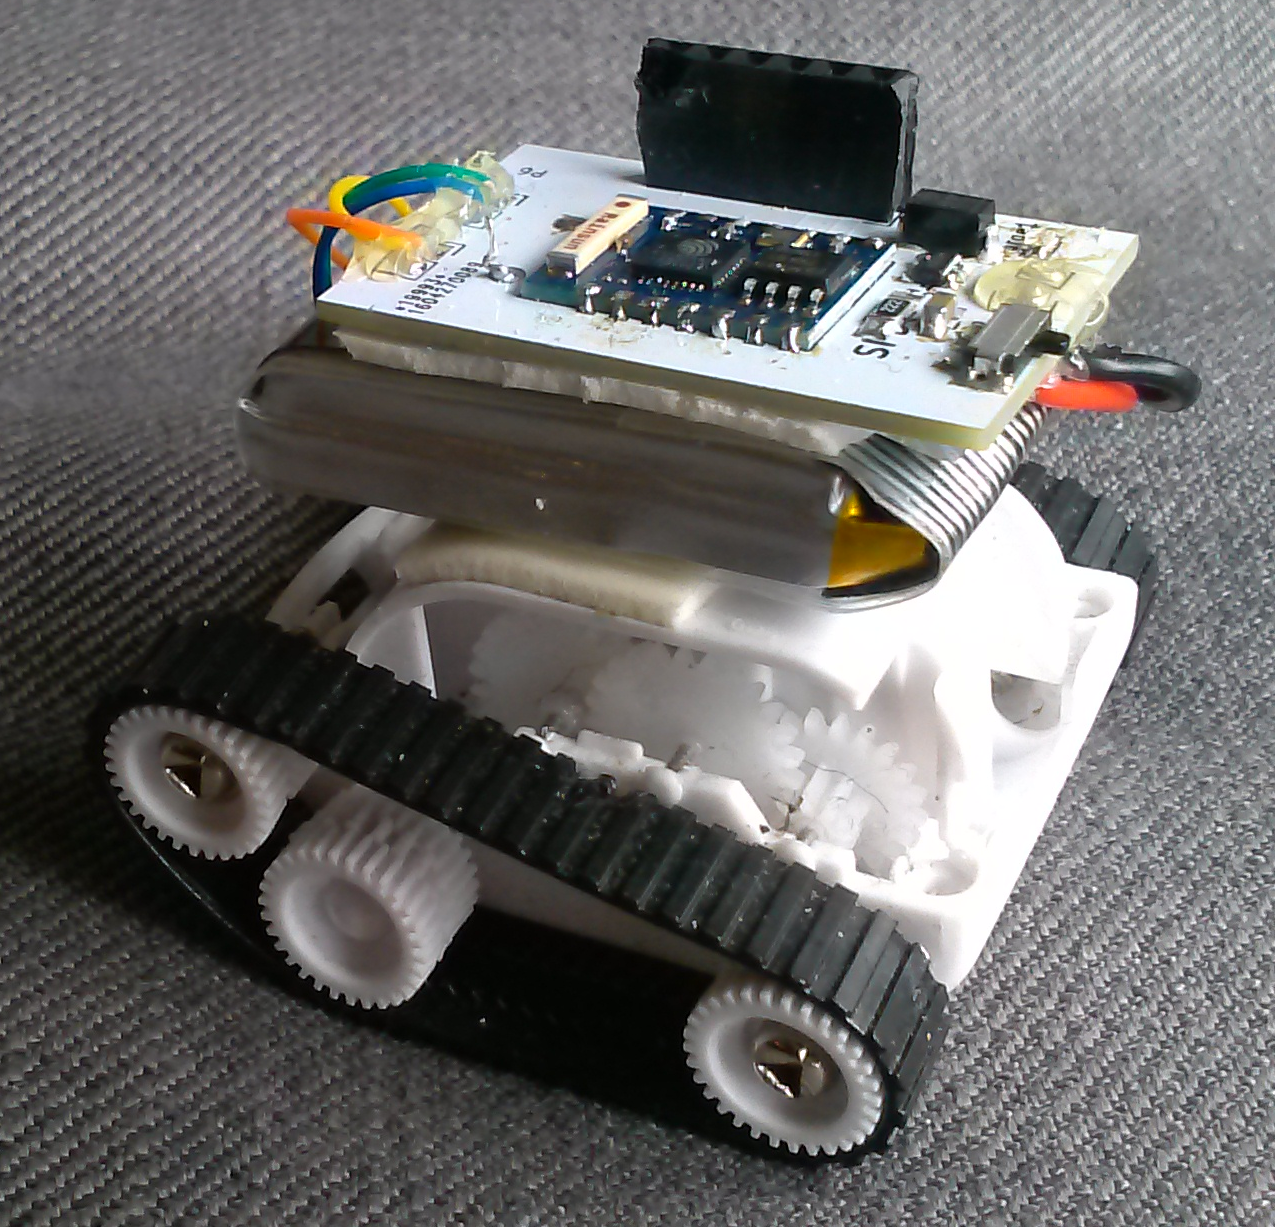
\includegraphics[width=0.8\textwidth]{../robot_makers_2/tiny_tank}
\caption{A tank-drive toy with a 3.7V lithium polymer battery and a control board mounted to it.}
\end{figure}

In order to be both heterogeneous and inexpensive, the robots used for this work are constructed by developing a Commercial Off-The-Shelf (COTS) modular control hardware platform that can be attached to children's toys. 
Modified toys are an adequate substitute for custom mechanical assemblies, and permit easy experimentation with heterogeneous swarms. 
The use of children's toys as mobility platforms may also avoid the sensitivity to the work surface exhibited by the Kilobots and, to a lesser extent, the Epucks.
The controller module was designed to be used as a replacement for the control electronics of children's toys, similar to the Spider-Bots developed by Laird, Price, and Raptis, or Bergbreiter's COTSBots \cite{lairdspider, bergbreiter2003cotsbots}.
However, unlike the Spider-Bots and COTSBots, this work does not specify a particular toy chassis to use for mobility. 
Most children's toys use either one motor with a mechanical linkage to cause the toy to turn when the motor is reversed, or two motors.
Two-motor toys frequently use either differential steering or have one motor provide drive power and the other provide steering. 
All of these toys can be controlled by the hardware described in this work. 

The robots are intended to be heterogeneous, partly because of the advantages of heterogeneity in a swarm, and partly because toy supplies are unreliable.
While toys in the general case are expected to remain available, a particular line of toys might be discontinued or a modified version released. 
The software framework in development to support the robots is based on ROS, and so allows modular replacement of the control algorithms used to convert desired motion of the robot into drive signals for the motors. 

%Toys cost $24, $16, $15, $21/2, 
\begin{table}
	\begin{tabular}{l l l l}
	Part & Price & Quantity & Subtotal\\
	\hline
	Mobile Toy & 14-20 & 1 & 20 \\
	Battery & 2.54 & 1 & 2.54 \\
	Main PCB & 2.75 &  1 & 2.75 \\
	ESP8266 Module & 2-7 & 1 & 7.0 \\
	DRV8830 & 2.30 & 2 & 4.60 \\
	MIC5319-3.3YD5 & 1.36 & 1 & 1.36 \\
	MCP73831 & 0.58 & 1 & 0.58 \\
	\hline
	Total & & & 27.83-38.83\\
	\end{tabular}
	\caption{All prices are for single quantities of new parts. It may be possible to get bulk discounts, especially on the toys and ESP-8226 modules. The costs of the resistors and capacitors has been left off, as they cost fractions of a penny each.}
\end{table}

The processor of the controller is an ESP-8266 wifi module.
The ESP-8266 costs approximately \$3-5, and contains both a wireless interface and a micro controller that can be programmed from a variety of programming environments and languages, including Lua and the Arduino variant of C/C++. The ESP-8266 module is based on the ESP-8266 IC, made by Expressif Systems. The IC itself has an 80Mhz Tensilica Xtensa L106 processor with 64kB of instruction memory and 96kB of data RAM. The modules come equipped with 512kB to 16MB of flash memory for program storage, and some combination of the 16 GPIO lines of the IC available for use. 
The ESP-8266 is available in several form factors, each designated by a different suffix. 
The version selected is the ESP-8266-03, which offers more GPIO pins than most other versions, and includes an internal antenna.

In addition to 802.11 b/g/n WiFi, the ESP-8266 supports a variety of serial protocols, including a UART, I$^2$C, SPI. 
The I$^2$C interface is used on the board to connect to two DRV8830 motor driver ICs by Texas Instruments. 
The DRV8830 provides 1A of drive current.
Experimental tests with 8 different toys indicate that small toys draw well under 1A while moving freely, and peak around 2A when the motors are stalled. 
The tested toys include 3 insect-styled walkers, 3 wheeled vehicles (2 differential drive, 1 Ackerman steering), 1 toy helicopter, and 1 toy quadcopter.
The DRV8830 provides overcurrent limiting, so a stall condition or short circuit of the motor leads will disable the motor drive, but not damage the DRV8830. 

The control module also provides connections for a 3.7V lithium-ion battery pack, as well as charge control circuitry for the battery. 
The charge controller allows the robot to be charged from the same USB connection that is used to change the programming of the ESP-8266. 
Reset and entry into programming mode is controlled by a separate USB-to-serial adapter board, the Sparkfun BOB-11736.
Moving this functionality to the adapter board reduces the size and cost of the control module. 

\subsection{Toy Compatibility}

Children's toys normally use inexpensive brushed DC motors in their construction. 
These motors have not been the subject of extensive study, as they are commodity parts. 
However, it is useful to quantify their behavior to some extent, to determine which kinds of toys can be used with the controller. 

Two common types of motors found in children's toys are the RE and FA series of motors produced by Mabuchi Motor, or imitations of these motors produced by other companies. 
These motors use simple metal brushes and are constructed to be inexpensive, rather than precise. 
The intended voltage range of the motors varies with different winding types, but according to datasheets available from Mabuchi Motor, the voltage ranges and current draws for motors in this range are as shown in table \ref{tab:properBrandedMotors}.

\begin{table}
	\begin{tabular}{l l l l l}
	Model & Voltage & No Load Current & Max Efficiency & Stall Current\\
	\hline
	RE-140RA-2270 & 1.5-3 & 0.21 & 0.66 & 2.1 \\
	RE-140RA-18100 & 1.5-3 & 0.13 & 0.37 & 1.07 \\
	RE-140RA-12240 & 3-6 & 0.05 & 0.14 & 0.39 \\
	FA-130RA-2270 & 1.5-3 & 0.2 & 0.66 & 2.2\\
	FA-130RA-18100 & 1.5-3 & 0.15 & 0.56 & 2.1\\
	FA-130RA-14150 & 1.5-4.5 & 0.11 & 0.31 & 0.9\\
	\end{tabular}
	\caption{Current draw for Mabuchi-branded motors.}
	\label{tab:properBrandedMotors}
\end{table}

These are somewhat large brushed motors. 
For smaller toys, coreless motors are more common. 
The values in table \ref{tab:coreless} were measured from six of the toys used in constructing the swarm.
The measurements from the toy helicopter and toy quadcopter are included for comparison.
While the board can supply sufficient current to control all of these toys, it has not been tested in flying platforms.

\begin{table}
	\begin{tabular}{l l l}
	Motor number & No Load Current & Stall Current (measured)\\
	\hline 
	Hexbug brand mini spider & 0.03A & 0.13A* \\
	Hexbug brand 6-legged insect & 0.06A & 0.25A \\
	Miniature toy RC car & 0.21A & 0.8A \\
	Miniature toy RC insect & 0.19A & 1.13A \\
	Miniature toy RC vehicle & 0.37A & 0.8A \\
	Miniature toy RC vehicle & 0.06A & 0.74A \\
	Toy helicopter & 0.07A & 1.12A \\
	Toy quadcopter & 0.74A & 1.99A \\
	\end{tabular}
	\caption{No load and stall current for coreless DC micromotors. Measurements were performed at 3V supply voltage. *The Hexbug mini spider includes a slip clutch, so attempting to stall the motors by holding the toy still does not prevent the motor from turning}
	\label{tab:coreless}
\end{table}


\subsection{Potential for Expansion}

The current design for the robots does not include sensors as a cost-saving decision. 
However, the communication between the ESP-8266 and the motor drivers uses the industry standard I2C bus serial interface. 
Due to the non-proprietary nature of this interface standard, it has been widely adopted, and many sensors are available to connect to an I2C bus. 
For example, Vishay Semiconductor makes the VCNL3020, which is an infrared proximity sensor with a 20mm range. 
If greater range is required, The ST Microelectronics VL53L0X Time-of-flight (ToF) laser ranger and gesture sensor provides a 2M range and 1D gesture sensing in a 4.4mm x 2.4mm package. 
As of this writing, the VCNL3020 is \$3.44 and the VL53L0X costs \$6.28 in single quantities.
These prices are reduced significantly when buying components in bulk, but because they increase the cost, size, and power draw of the hardware, they have not yet been integrated with this platform. 
Numerous multichannel ADC ICs with I2C interfaces are also available, which permits the addition of analog sensors to the platform. 


\bibliography{swarm.bib}
\bibliographystyle{apalike}

\end{document}

%Papers to read

%Cooperative interaction of walking human and distributed robot maintaining stability of swarm 

%Development of IR-based short-range communication techniques for swarm robot applications 

%The Wanda Robot and Its Development System for Swarm Algorithms

%Stability of swarm robot based on local forces of local swarms

%Swarm robot pattern formation using a morphogenetic multi-cellular based self-organizing algorithm 

%A particle-swarm-optimized fuzzy-neural network for voice-controlled robot systems 

%The I-SWARM project 
%
%\subsection{Current Consumption of Children's Toys}
%Motor driver test required, a well as quantification of motor current draw for children's toys. 
%Quantification of required power may indicate that larger motor driver power is needed.
%
%Toys are effectively black boxes to the end user.
%Motors in particular are a commodity item, manufactured in large quantities without particular demand for electrical efficiency. 
%In the toys \improvement{Photos of motors and toys} used in this work, the most common motors are coreless brushed DC motors, although some of the larger toys also used brushed DC motors with cores. 
%The presence or absence of a core in the motor is of little practical concern in toys or in swarm robotic applications, as they are driven identically. 
%
%All of the motors were driven at 3.7VDC. 
%This voltage was chosen because it is the output voltage of a fully-charged COTS lithium-polymer battery, which the platform uses for power. 
%Current was recorded for each motor running without the robot being in contact with the ground, to assess the minimum current draw, and stalled, to determine the potential maximum draw. 
%Current was measured using a multimeter, which does not have storage or recording capability, and so no attempt was made to determine peak surge current. 
%
%Hexbug brand mini spider (two coreless brushed DC motors) Free run: 0.03A    Stall: 0.13A
%Hexbug brand 6-legged insect (one coreless brushed DC motor) Free run: 0.06A    Stall: 0.25A
%Miniature toy RC car, unknown model (one coreless brushed DC motor) Free run: 0.21A   Stall: 0.8A
%Miniature toy RC insect, unknown model (two motors, unknown construction) Free run: 0.19A    Stall: 1.13A
%Miniature toy RC car, differential steering (two motors, unknown construction) Free run: 0.37A    Stall: 0.8A
%Miniature toy RC vehicle, differential steering (two motors, unknown construction) Free run: 0.06A    Stall: 0.74A
%Toy helicopter (two motors, unknown construction, probably brushless) Free run: 0.07A   Stall: 1.12A
%Toy quadcopter (four motors, unknown construction, probably brushless) Free run: 0.74A   Stall: 1.99A
